\documentclass[11pt, oneside]{article} 
\usepackage{geometry}
\geometry{letterpaper} 
\usepackage{graphicx}
	
\usepackage{amssymb}
\usepackage{amsmath}
\usepackage{parskip}
\usepackage{color}
\usepackage{hyperref}

\graphicspath{{/Users/telliott//Github/calculus_book/png/}}
% \begin{center} 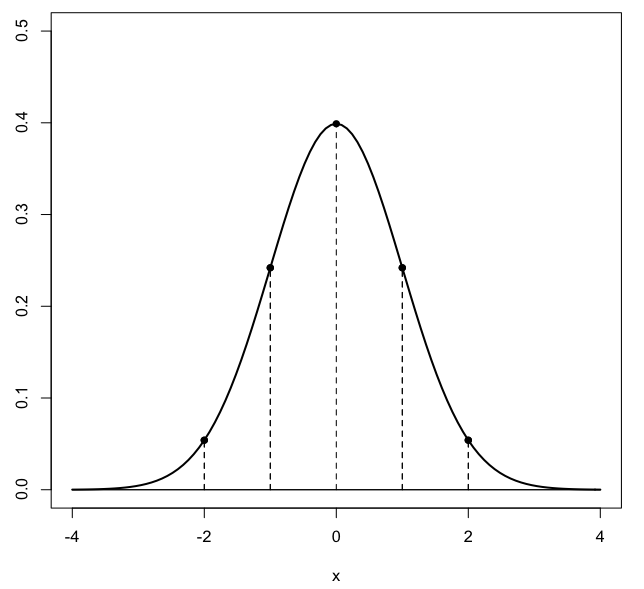
\includegraphics [scale=0.4] {gauss3.png} \end{center}

\title{Factor of one third}
\date{}

\begin{document}
\maketitle
\Large

\label{sec:one_third}

Knowing basic calculus allows us to see intuitively where the factor of one-third comes from in the formula for the volume of a pyramid or a cone.  It comes from integrating $x^2 \ dx$ and obtaining $x^3/3$.

However, it is interesting to see how things might have been discovered in the age before calculus.

\subsection*{algebraic derivation of the constant 1/3}

I found an algebraic argument on the web at 

\url{https://web.maths.unsw.edu.au/~mikeh/webpapers/paper47.pdf}

Let us assume for this proof that the volume of a cone is proportional to both the area of the base and the height:  $V = cAh$;  our objective is to find the constant of proportionality.

It takes a bit of algebra to see, but gives the value for the proportionality constant as $1/3$.

Consider a conical frustum, a cone with the top lopped off.  

\begin{center} 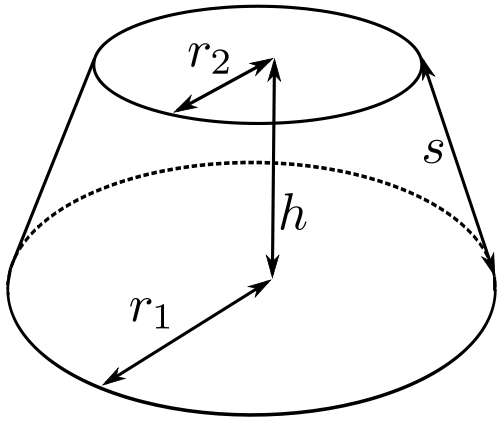
\includegraphics [scale=0.4] {conical_frustum.png} \end{center}

Suppose the area of the base is $A$ and the height of the frustum is $h$.  

Calculate the volume of the frustum as the difference between that of a larger cone with base $A$ and height $h + e$ (e for extra), and that of a small cone with base area $a$ and height $e$.

\[ V = cA(e + h) - cae \]

Now, the area of the base of a cone is $\pi$ times the radius squared, and the radius is proportional to the height (depending on the slant angle).  Hence
\[ a = ke^2 \]
The area of the small base is proportional to the height squared, and the same for the large one:
\[ A = k(e + h)^2 \]
so
\[ k = \frac{a}{e^2} =\frac{A}{(e+h)^2} \]
Hence
\[ \frac{\sqrt{a}}{e} = \frac{\sqrt{A}}{e + h} \]

Let us manipulate this expression to find $e$ in terms of $h$:
\[ \frac{\sqrt{A}}{\sqrt{a}} = 1 + \frac{h}{e} \]
\[ \frac{h}{e} = \frac{\sqrt{A} - \sqrt{a}}{\sqrt{a}} \]
\[ e = \frac{\sqrt{a}}{\sqrt{A} - \sqrt{a}} \cdot h \]

And then
\[ e + h = \frac{\sqrt{A}}{\sqrt{A} - \sqrt{a}} \cdot h \]

Substituting into what we had above for the volume:
\[ V = cA(e+h) - cae \]
\[ = cA \ [ \frac{\sqrt{A}}{\sqrt{A} - \sqrt{a}} \cdot h \ ] - ca \ [ \frac{\sqrt{a}}{\sqrt{A} - \sqrt{a}}  \cdot h \ ] \]
\[ = c \ [ \   \frac{A \sqrt{A} - a \sqrt{a}}{\sqrt{A} - \sqrt{a}} \ ] h \]

This looks like a mess.  But it is really $(m^3 - n^3)/(m-n)$  Factoring the numerator we get $m^2 + mn + n^2$.  That is:

\[ V = c (A + \sqrt{A} \sqrt{a} + a) h \]

Let $a \rightarrow A$.  That is, consider what happens as $a$ gets larger and closer to $A$. The expression in parentheses becomes $3A$.  Hence:
\[ V = c(3A)h \]
But as $a \rightarrow A$ the frustum becomes a cylinder whose volume we know is equal to $Ah$. 
\[ V = c(3A)h = Ah \]

Therefore $c = 1/3$.

$\square$

\end{document}